% =====================================================================
%  Entregable T3(a): Muchos cuerpos por trayectorias cuanticas (MPI)
%  Fragmento \input-able en context/doc/mpemba_cuantico.tex
% =====================================================================
\section{Muchos cuerpos: trayectorias cuánticas con MPI}
\label{sec:t3}

\subsection{Explicación del framework}
En el régimen de \emph{muchos cuerpos} la representación densa del operador
densidad $\rho$ se vuelve inviable: para $N$ qubits, $\rho$ tiene $d^2=4^N$
elementos y el Liouvilliano $4^N\times4^N$. El método de \textbf{trayectorias
cuánticas} (\emph{Monte Carlo wavefunction}, MCWF) sortea este muro: en lugar de
propagar $\rho$, propaga $M$ \emph{vectores de estado puros}
$\ket{\psi}\in\mathbb{C}^{d}$ y recupera el operador densidad como promedio
estocástico
\[
\rho(t)=\mathbb{E}\big[\dyad{\psi(t)}{\psi(t)}\big]\;\approx\;\frac1M\sum_{j=1}^{M}\dyad{\psi_j(t)}{\psi_j(t)}.
\]
Esto reduce la memoria de $d^2$ a $d$ y, sobre todo, convierte el problema en uno
\textbf{embarrassingly parallel}: cada trayectoria es independiente.

\subsection{Del modelo teórico a la discretización (paso a paso)}
\label{ssec:t3_discr}

\paragraph{Paso 0 — Modelo teórico.} El mismo generador GKSL
$\dot\rho=\Lop[\rho]$ de la cadena de Ising disipativa (\S\ref{ssec:t2a_discr}).

\paragraph{Paso 1 — \emph{Unraveling} estocástico.} En vez de propagar $\rho$, se
reescribe la ecuación maestra como un promedio sobre \emph{trayectorias} de
estados puros (\emph{Monte Carlo wavefunction}, Dalibard--Mølmer--Castin):
$\rho(t)=\mathbb{E}\big[\dyad{\psi(t)}{\psi(t)}\big]$. La parte coherente más la
parte ``de no salto'' del disipador se agrupan en un \textbf{Hamiltoniano efectivo
no hermítico}
\[
H_{\mathrm{eff}}=H-\tfrac{i}{2}\sum_\mu L_\mu^\dagger L_\mu,
\]
cuya evolución $\dot{\ket\psi}=-iH_{\mathrm{eff}}\ket\psi$ \emph{no} conserva la
norma; el defecto de norma es exactamente la probabilidad de salto.

\paragraph{Paso 2 — Discretización temporal de cada trayectoria.} Con paso
$\Delta t$, cada trayectoria alterna:
\begin{enumerate}[leftmargin=1.6em,itemsep=1pt]
\item \textbf{Evolución determinista} $\dot{\ket\psi}=-iH_{\mathrm{eff}}\ket\psi$ por
\textbf{RK4} (4.º orden; elimina el sesgo $\mathcal{O}(\Delta t)$ de un Euler
ingenuo). Resulta $\psi'$ con $\|\psi'\|^2=1-\delta p$.
\item \textbf{Salto estocástico.} Probabilidad $\delta p=1-\|\psi'\|^2$; se sortea
$\varepsilon\sim U(0,1)$: si $\varepsilon<\delta p$ hay \emph{salto} (se elige el
canal $\mu$ con probabilidad $\propto\|L_\mu\psi\|^2$ y
$\ket\psi\leftarrow L_\mu\ket\psi/\|L_\mu\psi\|$); si no,
$\ket\psi\leftarrow\psi'/\|\psi'\|$.
\end{enumerate}

\paragraph{Paso 3 — Promedio de conjunto.} El observable se recupera promediando
las $M$ trayectorias,
$\rho(t)\approx\frac1M\sum_{j=1}^{M}\dyad{\psi_j(t)}{\psi_j(t)}$. Coste por paso:
unos pocos productos matriz--vector $\mathcal{O}(d^2)$ (no $\mathcal{O}(d^3)$);
precisión del promedio $\propto M^{-1/2}$. \emph{Las $M$ trayectorias son
independientes} $\Rightarrow$ el promedio es la única operación colectiva
(Paso~3 $=$ una \texttt{MPI\_Reduce}).

\subsection{Implementación serial y líneas de código}
En \texttt{T3/integration/src/trajectories\_mpi.cpp} (reutiliza
\texttt{T2/common/lindblad.hpp} para el modelo y \texttt{matvec}). El estado
inicial es el puro $\ket{0}$ y la referencia el Gibbs del baño. Cada trayectoria
usa un generador \texttt{mt19937\_64} sembrado con su índice \emph{global}, lo que
hace el resultado \textbf{reproducible e independiente del número de rangos}. El
Paso~2 (no-salto vs salto) es literalmente:

\begin{lstlisting}[language=C++,caption={Decisión determinista/salto por trayectoria (\texttt{trajectories\_mpi.cpp}). \texttt{psip} es el estado tras el paso RK4 de $H_{\mathrm{eff}}$; \texttt{norm2}$=\|\psi'\|^2$.},label={lst:t3_jump}]
double dp = 1.0 - norm2;                              // probabilidad de salto
if (U(rng) < dp) {                                    // --- SALTO ---
    /* elegir canal mu con prob ~ ||L_mu psi||^2 ... */
    std::vector<cd> Lp = matvec(Ls[mu], psi, d);
    for (int a = 0; a < d; ++a) psi[a] = Lp[a] / nn;  // psi <- L_mu psi / ||.||
} else {                                              // --- NO salto: renormalizar ---
    double inv = 1.0 / std::sqrt(norm2);
    for (int a = 0; a < d; ++a) psi[a] = psip[a] * inv;
}
\end{lstlisting}

\subsection{Las llamadas de paralelización (MPI)}
El paralelismo es de \emph{tareas}: cada rango calcula su lote de trayectorias sin
comunicación, y una sola reducción promedia. Las tres líneas MPI que estructuran
todo el cálculo son el arranque, el reparto y la reducción final:

\begin{lstlisting}[language=C++,caption={Esqueleto MPI de \texttt{trajectories\_mpi.cpp}: arranque e identificación del rango, reparto balanceado de las $M$ trayectorias entre rangos (sin comunicación), y la \emph{única} operación colectiva \texttt{MPI\_Reduce} que suma los acumuladores en el rango 0 (Paso~3, el promedio).},label={lst:t3_mpi}]
MPI_Init(&argc, &argv);                       // arranque del entorno MPI
MPI_Comm_rank(MPI_COMM_WORLD, &rank);         // id de este rango
MPI_Comm_size(MPI_COMM_WORLD, &size);         // numero total de rangos
// ... reparto balanceado de las M trayectorias (embarrassingly parallel):
int per = M / size, rem = M % size;
int my_M = per + (rank < rem ? 1 : 0);        // cuantas calcula este rango
int my_start = rank * per + std::min(rank, rem);
// ... cada rango integra sus my_M trayectorias en un acumulador local 'acc' ...
// UNICA comunicacion: sumar los acumuladores locales -> rho(t) en el rango 0
MPI_Reduce(reinterpret_cast<double*>(acc.data()),
           rank == 0 ? reinterpret_cast<double*>(glob.data()) : nullptr,
           (int)(2 * acc.size()), MPI_DOUBLE, MPI_SUM, 0, MPI_COMM_WORLD);
\end{lstlisting}

\subsection{Justificación de la paralelización: MPI}
El patrón de cómputo es radicalmente distinto al de la evolución temporal (T2):
no hay una larga cadena de pasos dependientes sobre un único objeto grande, sino
$M$ cálculos \emph{completamente independientes} sobre objetos pequeños
($\ket\psi\in\mathbb{C}^d$), seguidos de una \emph{única reducción} (el promedio).
Este es el caso de libro del paradigma \textbf{MPI} de paralelismo de tareas:
cada rango calcula su lote de trayectorias sin comunicación alguna y al final una
sola \texttt{MPI\_Reduce} promedia los acumuladores. No hay comunicación de halo
ni dependencias, por lo que el escalado es \emph{casi ideal} y \emph{multinodo}
(a diferencia de OpenMP, limitado a un nodo y al ancho de banda compartido).
CUDA sería un acelerador complementario \emph{dentro} de cada rango (evolucionar
cientos de trayectorias en lote en una GPU), pero el reparto grueso natural es
MPI. La corrección se verifica de dos formas: (i)~el resultado es idéntico con
1, 4 u 8 rangos (misma semilla por índice global $\Rightarrow$ reducción
correcta); (ii)~el promedio reproduce la ecuación maestra exacta (validación
abajo).

\subsection{Comparación serial vs paralelo}
\begin{figure}[h]
\centering
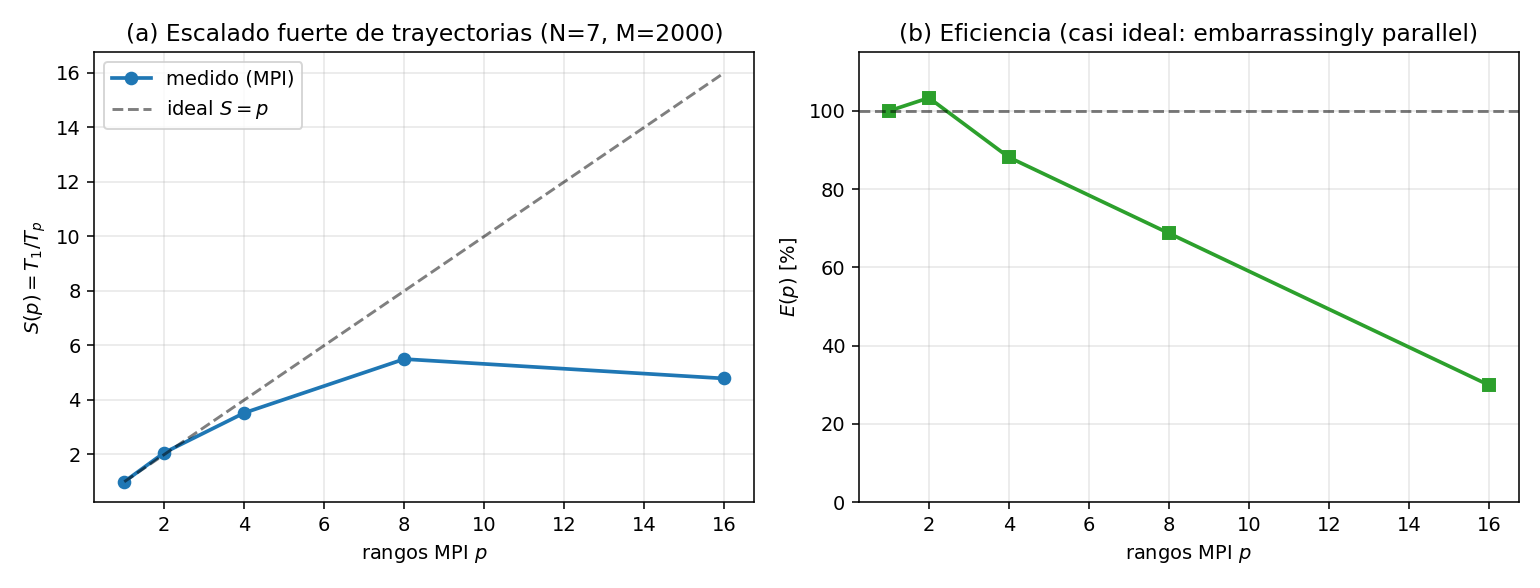
\includegraphics[width=0.92\textwidth]{../../T3/integration/results/fig_t3_speedup.png}
\caption{Escalado fuerte de las trayectorias cuánticas sobre rangos MPI
($N=7$, $M=2000$ fijo). El speedup es \textbf{casi ideal}
($S_{\max}\approx5{,}5$ con $8$ rangos, eficiencia $69\,\%$),
en marcado contraste con el escalado sublineal del OpenMP de la evolución
temporal (T2, $S\approx2{,}9$--$3{,}3$). La razón: ausencia total de
comunicación y dependencias entre trayectorias.}
\label{fig:t3_speedup}
\end{figure}

\textbf{Contraste de paradigmas (el resultado clave del reparto T2 vs T3).} La
evolución temporal (T2) paraleliza \emph{dentro} de un paso con OpenMP y satura
pronto (memoria compartida, ancho de banda, fork/join): $S\!\lesssim\!3{,}3$. Las
trayectorias (T3) paralelizan \emph{entre} tareas independientes con MPI y escalan
casi linealmente: $S\approx5{,}5$. Es la ilustración perfecta de que el
paradigma óptimo lo dicta el \emph{patrón de cómputo}, no una preferencia a
priori.

La Figura~\ref{fig:t3_serial_parallel} hace explícita la mejora variando el
parámetro propio del método —el \textbf{número de trayectorias $M$}, que fija el
trabajo Monte Carlo— y enfrentando el \textbf{tiempo en serie (1~rango) y en
paralelo (8~rangos)}. Ambas crecen linealmente con $M$ (coste $\propto M$), pero
con pendientes muy distintas: las rectas \emph{divergen}, y el cociente entre
ellas se mantiene casi constante y cercano al número de núcleos, precisamente
porque no hay comunicación entre trayectorias.

\begin{figure}[h]
\centering
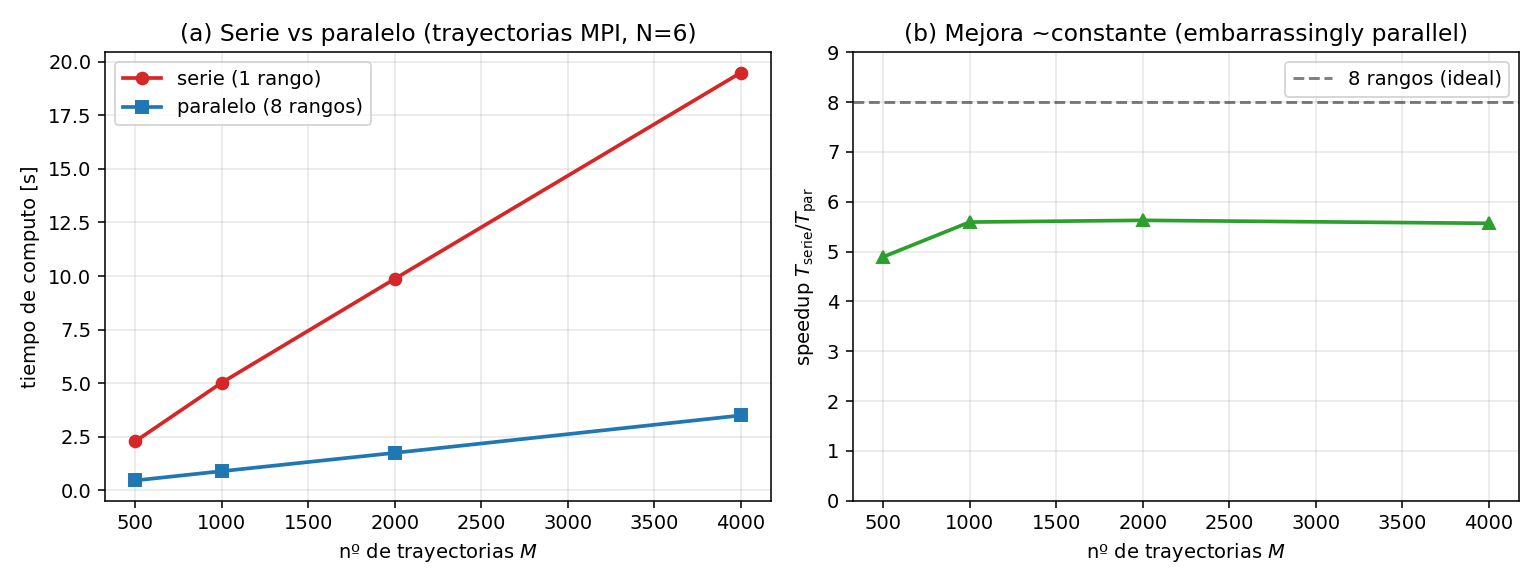
\includegraphics[width=0.92\textwidth]{../../T3/integration/results/fig_t3_serial_parallel.png}
\caption{Tiempo de cómputo \textbf{serie vs paralelo} de las trayectorias frente
al número de trayectorias $M$ ($N=6$, $d=64$). (a)~serie ($1$~rango, rojo) y
paralelo ($8$~rangos, azul) crecen como $\propto M$ con pendientes distintas: el
hueco —la mejora— se ensancha con $M$. (b)~el speedup
$T_{\mathrm{serie}}/T_{\mathrm{par}}$ es \emph{casi constante} en $M$ (línea de
referencia ideal $=8$), firma del paralelismo \emph{embarrassingly parallel}.}
\label{fig:t3_serial_parallel}
\end{figure}

\subsection{Resultados y validación}
\paragraph{Convergencia estadística.}
La figura~\ref{fig:t3_error} muestra que el error del observable $D_{HS}$ final frente a
la ecuación maestra exacta (evolución espectral desde $\ket{0}$,
$D_{HS}^{\text{exacto}}=0{,}40490$) decae como $M^{-1/2}$ (pendiente medida
$\approx-0{,}6$, consistente con $M^{-1/2}$), confirmando la convergencia de Monte Carlo. El uso de RK4 en
la parte determinista elimina el sesgo sistemático: a $\Delta t=0{,}02$ y
$M=8000$ el resultado coincide con el exacto con una diferencia de $\sim0{,}002$.

\begin{figure}[h]
\centering
\begin{minipage}{0.49\textwidth}\centering
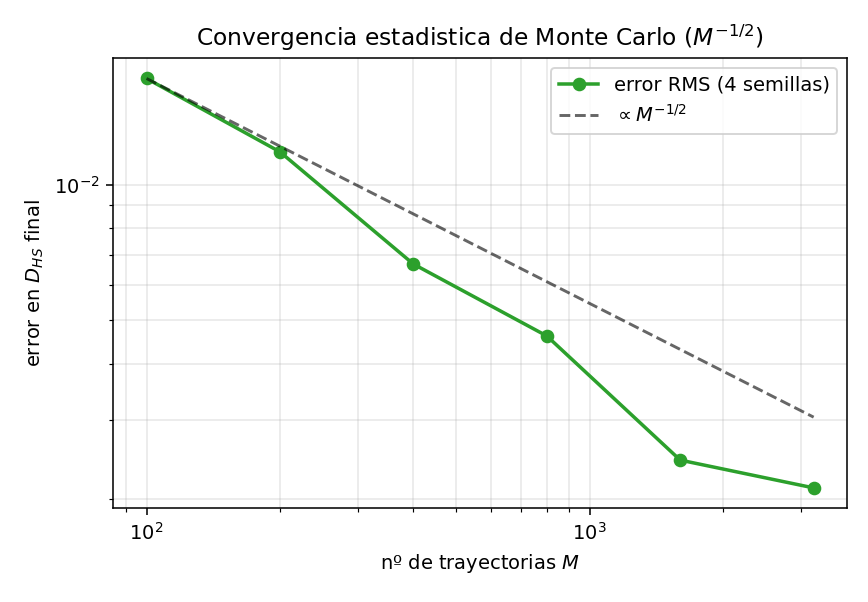
\includegraphics[width=\textwidth]{../../T3/integration/results/fig_t3_error_M.png}
\end{minipage}\hfill
\begin{minipage}{0.49\textwidth}\centering
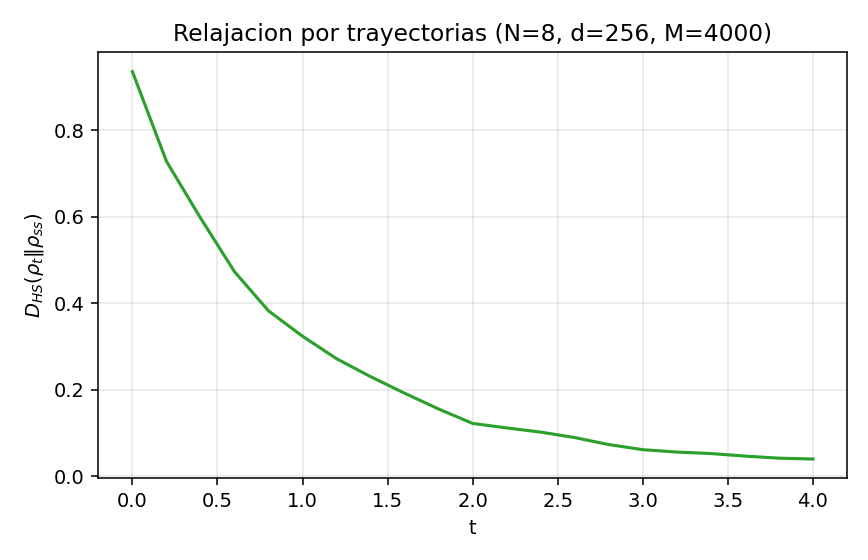
\includegraphics[width=\textwidth]{../../T3/integration/results/fig_t3_relax.png}
\end{minipage}
\caption{Izquierda: convergencia estadística $M^{-1/2}$ del promedio de
trayectorias. Derecha: curva de relajación $D_{HS}(t)$ para $N=8$ ($d=256$,
$M=4000$), un sistema en el que el método de trayectorias usa vectores de $256$
componentes en lugar de operadores densidad de $256^2$.}
\label{fig:t3_error}
\end{figure}

\paragraph{Conclusión del método de trayectorias.}
Las trayectorias cuánticas son el método de elección para muchos cuerpos: memoria
$\mathcal{O}(d)$ por trayectoria, coste $\mathcal{O}(d^2)$ por paso y, sobre todo,
\textbf{escalado MPI casi ideal} que aprovecha clústeres multinodo. El precio es
la convergencia $M^{-1/2}$ (para una cifra más de precisión hacen falta $100\times$
trayectorias), mitigable precisamente por la abundancia de paralelismo. Para
cadenas largas y observables de entrelazamiento, el relevo natural son las redes
tensoriales (entregable de Juan, \S\ref{sec:t3b}).
